\documentclass{article}
\usepackage{url}
\usepackage{graphicx}
\usepackage{fancyhdr}
\usepackage{hyperref}
\usepackage{listings}
\lstset{ %
  language=C,            	% the language of the code
  basicstyle=\ttfamily,       	% the size of the fonts that are used for the code
  showspaces=false,           	% show spaces adding particular underscores
  showstringspaces=false,     	% underline spaces within strings
  showtabs=false,    	         % show tabs within strings adding particular underscores
  tabsize=2,                  	% sets default tabsize to 2 spaces
  captionpos=b,               	% sets the caption-position to bottom
  breaklines=true,            	% sets automatic line breaking
  breakatwhitespace=false    	% sets if automatic breaks should only happen at whitespace
}
\begin{document}
 
\special{papersize=8.5in,11in}
\setlength{\paperheight}{11in}
\setlength{\paperwidth}{8.5in}
\setlength{\pdfpageheight}{\paperheight}
\setlength{\pdfpagewidth}{\paperwidth}
 
\title{Fluid Photo Browser with\\NFC-based Payment and Printed Photo Pickup}
\author{
  David Thomas (dtho@itu.dk)\\
  Egil Hansen (ekri@itu.dk)\\
                         	Jonas Rune Jensen (jruj@itu.dk)}
\maketitle
 
\section{Introduction}
The task for this assignment was to develop a tabletop app for a photo print shop, featuring transfer of photos between the tabletop and customers' smartphones of as well as payment for printed photos using Near-Field Communication (NFC). The tabletop app should allow editing of the photos before printing them and sending them back to the customer.
 
\section{Background}
 
\subsection{Tabletop computing}\label{tabletopTheory}
Tabletop computing generally covers the use of large, horizontally-mounted touch screens. As described in \cite{integratingTechnology}, this encourages usage which differs from the white board-inspired use of wall-mounted displays. Tabletop computers are often surrounded by people interacting from different angles.
 
\section{The System}
The system we have implemented consists of the parts shown in figure \ref{fig:deployment-diagram}: the tabletop app itself, an Android app for the customers, a service  on Google App Engine to facilitate communication between the tabletop app and the Android app, and finally a helper program to connect the tabletop to an NFC reader.
 
To summarize the scenario, the idea is that a customer enters a print shop and uploads one or more pictures to the shop's tabletop computer from an Android phone. The pictures are edited on the tabletop and sent back to the phone, and printouts of the pictures are paid for using an NFC-based payment system.
 
Each part is described in details in the following sections. The source code is available at \url{https://github.com/jeffton/Pervasive-Assignment-2}.
 
\begin{figure}[t]
                         	\begin{center}
                                                      	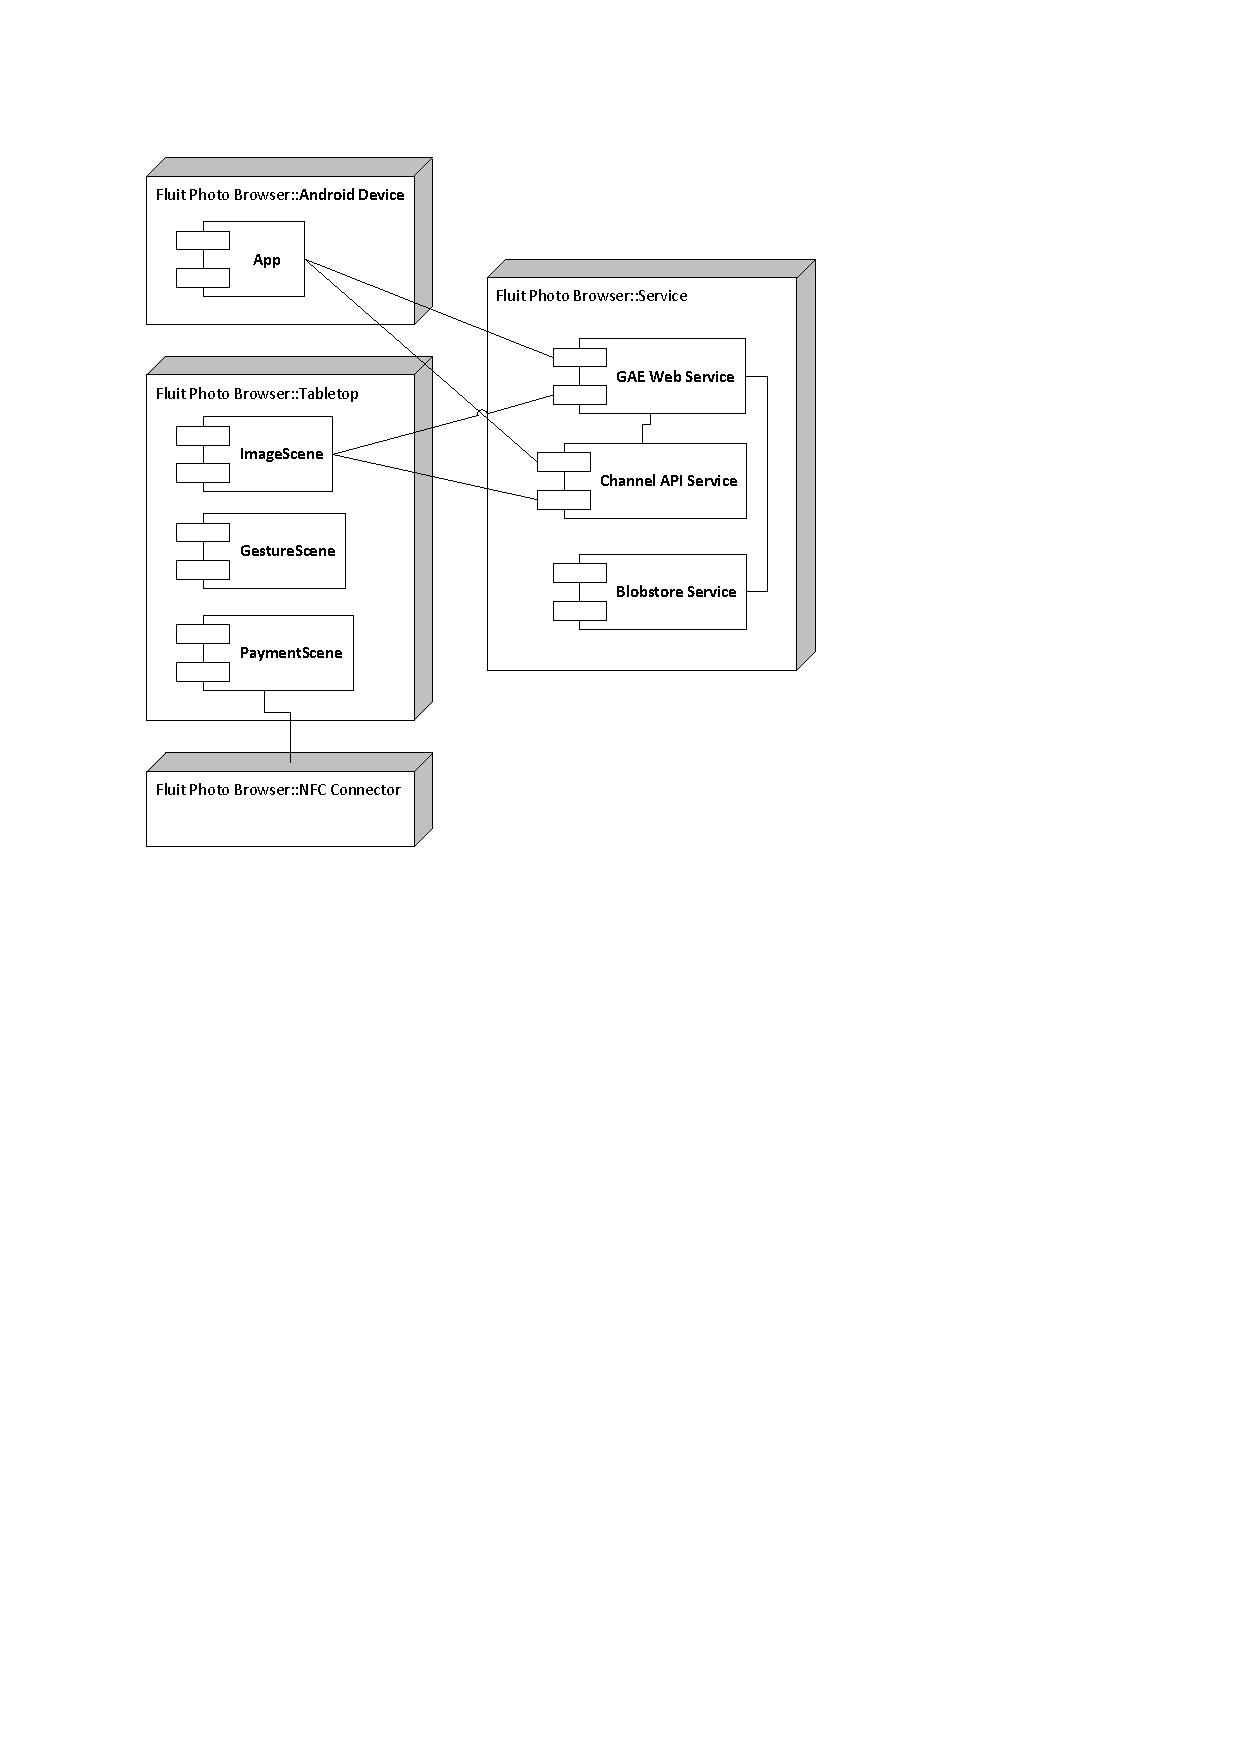
\includegraphics[width=0.8\textwidth]{deployment-diagram-fluit-photo-browser.pdf}
                         	\end{center}
                         	\caption{Deployment diagram for the system.}
                         	\label{fig:deployment-diagram}
\end{figure}
 
\section{Tabletop App}
MT4J \footnote{\url{http://mt4j.org}} is a Java-based framework for multitouch applications. MT4J apps consist of a number of scenes, of which ours has three. \lstinline{ImageScene}, shown in figure \ref{fig:image-scene}, displays images as they are uploaded from the phone and provides options for editing. Editing is kept within the same scene for simplicity and ease of use -- the last-tapped image is highlighted and will be the target of any applied effects. For our prototype, we have implemented a single effect: cropping.
 
\begin{figure}[t]
\begin{center}
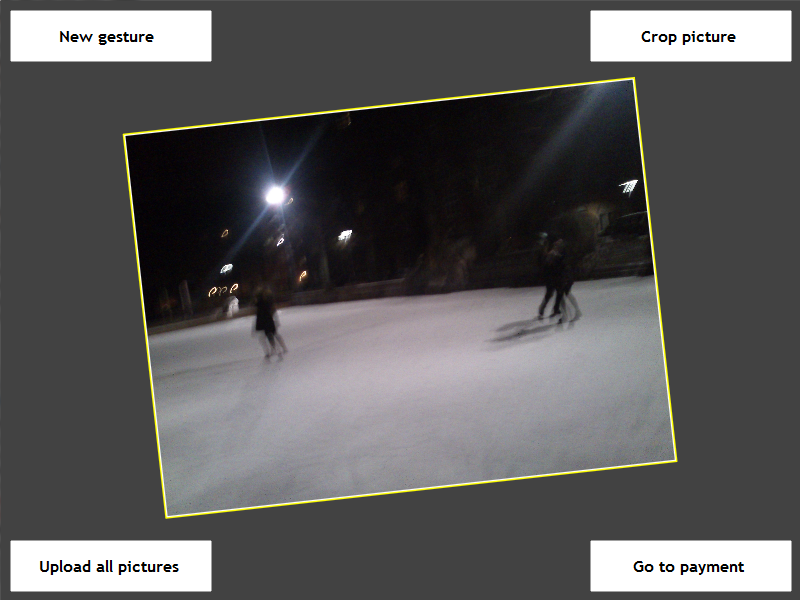
\includegraphics[width=0.8\textwidth]{image-scene.png}
\end{center}
\caption{\lstinline{ImageScene} in the Tabletop App.}
\label{fig:image-scene}
\end{figure}
 
After editing, the images can be sent back to the phone -- either by applying a custom gesture, or by tapping the upload button. The custom gesture can be defined by tapping `New gesture', which leads to the \lstinline{GestureScene}. Here, the user can define a gesture by recording a movement as a list of coordinates.
 
Finally, the \lstinline{PaymentScene} handles the payment flow. When an NFC card is connected, the balance is shown along with the number of pictures corresponding to the ID stored on the card. When accepting the payment, the balance on the card is reduced, and the user is returned to the image scene where the purchased images have been removed.
 
\subsection{Image Transfer}
All transfers of images between the tabletop app and the Android app happen through the Google App Engine service described in section \ref{service}. Since the tabletop app subscribes to notifications from the service, images appear on the tabletop almost instantly after being uploaded from the Android app.
 
\section{Android App}
The android application has two functions, upload selected pictures to the tabletop and downloading the edited pictures.
 
For selecting pictures we are using the Androids built in intent to select data on the device. In our case it is specified to be pictures. By using the built in intent, there is the disadvantage that we can only select one picture to upload at a time, which means that the user has to select upload button again for each picture. For a better user experience, we could build a custom intent where the user is able to select more than one picture.
 
When the user has selected a picture, it is uploaded to our service on Google App Engine, and then downloaded by the tabletop application.
 
When the tabletop is done editing the picture and uploads it to the service on Google App Engine, the application receives a push notification with id of the picture, and starts downloading it.
We save the downloaded picture in a folder called PicPush so we don't delete older pictures.
 
\section{Service on Google App Engine}\label{service}
 
The photo relay service\footnote{\url{http://fluid-photos-at-itu.appspot.com/}} we built is hosted on Google App Engine\footnote{\url{https://appengine.google.com/}} and gives us a few advantages over a hardcoded static IP during development, at the cost of a little more work, and it gave us a chance to build a system that is a little closer in design to a system one would build in the wild.
 
The main benefit is the loose coupling between the Android and tabletop app. They do not need to know about each other explicitly, and this allows the system to scale very easily, e.g. support more than one tabletop. Loose coupling also enables us to develop each component mostly independent of each other since each implementation just has to adhere to the agreed upon web service interface.
 
On the protocol level, using Google App Engine also means using HTTP(S) for transport of the photographs between it, the Android app, and the Tabletop app. Normally, HTTP only supports pulling for resources, but luckily Google has a solution for this as well called The Channel API\footnote{\url{https://developers.google.com/appengine/docs/java/channel/}}. The Channel API allows us to push notification from the photo relay service to the Android and Tabletop app when something of interest happens, such as a new photo being uploaded. With push notifications we are able to get very seamless transfer of photos between the apps.
 
The biggest downside of using the photo relay service is that the transfer time is increased, but we feel that the added transfer time is a fair tradeoff considering the benefits mentioned above.

\subsection{Photo Relay API}
 
\paragraph{Uploading a photograph}
To upload a photograph, a client must first calls \lstinline{/getUploadUrl}. A unique upload URL is required by the Google App Engine cloud storage system. With the new upload URL the client uses regular \lstinline{HTTP POST} to upload photo(s) along with an associated NFC ID and the source of the upload, ie. Android or tabletop.
 
\paragraph{Downloading}
The service provides two ways of querying for photographs, \lstinline{/getPhotoUrls} and \lstinline{getPhotoUrlsByNfcId?nfcid=<NFC ID>}. The latter allows clients to filter photographs by associated NFC ID. Querying either will result in a JSON array like to the example below:
 
\begin{lstlisting}
[
  {
  	"id":"AMIfv...",
    "source":"android",
    "filename":"DSC_0072.JPG",
    "nfcId":"123",
    "uploadedOn":1334853268514
  },
  {
    "id":"4VYNz...",
    "source":"android",
    "filename":"DSC_0054.JPG",
    "nfcId":"123",
    "uploadedOn":1334853971989
  }
]
\end{lstlisting}
 
With the ID of each photo, the client can now call \lstinline{ /getPhotoById?id=<photo id>} to get the raw photo data.
 
\paragraph{Deleting a photograph}
It is also possible to delete a photo stored in the cloud service. This is done via a call to \lstinline{ /deletePhotoById?id=<photo id>} with the ID of the photo.
 
\paragraph{Push notifications}
The clients must acquire a security token before they can subscribe to receive push notifications from the cloud service. This is done through a \lstinline{HTTP GET} call to the \lstinline{/token} service call. Once a client has a token, it can use a Google App Engine Channel Client framework to do the heavy lifting of keeping the communication channel open. In our case, we used the Tom Parker's Java AppEngine Channel Client framework\footnote{\url{http://masl.cis.gvsu.edu/2012/01/31/java-client-for-appengine-channels/}}.
 
\section{NFC Payment}
NFC technology is used for identification with the tabletop app as well as for payment. In our proof of concept, the payment takes place directly in the tabletop app. As we are lacking an NFC-enabled Android phone, a MiFare Classic NFC-card is used. We store information on blocks 1 and 2 on the card: block 1 contains a header and an ID, and the block 2 contains the amount of available coins.
 
Communication with the card is implemented in a C\# helper application using the C\# API in the PC/SC SDK from SpringCard \footnote{\url{http://www.springcard.com/download/sdks.html}}. The tabletop app starts this helper application in a separate process and communicates through standard input and output streams.
 
\section{Limitations}
 
\subsection{Lack of Security in the Payment System}
No attempts have been made to secure the payment system, so cloning a card as well as changing the amount stored on one is straightforward. Since the built-in encryption on MiFare Classic cards is insecure \cite{darkSide}, we should encrypt our data before storing it on the card. This would prevent tampering but not cloning. With an online system such as this one, security could be increased by storing the amount on a server rather than on the card itself. While this would not prevent cloning, it would prevent spending the same coins twice. To avoid the cloning problem completely, we could use one of the more secure - but more expensive - successors to the MiFare Classic card.
 
\subsection{Push Notifications on Android}
Instead of using the Channel API to get push notification from the Google App Engine, we could have used the Android Cloud to Device Messaging Framework\footnote{\url{https://developers.google.com/android/c2dm/}}. This framework pushes messages to the device using its connection to Google services. The most useful part, is that our app would not have to be open, as the device would automatically open the app and a give it the message to process. But we are not able to use the system with the tabletop, so we chose the Channel API as it works on both systems, and potential other new systems.
 
\subsection{Choice of NFC SDK}
The license of the SpringCard SDK restricts distribution to applications that use card readers purchased through SpringCard. Also, the C\# helper application limits the platform independence of our tabletop app. Nonetheless, the SDK works for our proof of concept, and the NFC commands would be the same for any SDK.
 
\section{Conclusion}
For this assignment, we have implemented a tabletop app for a photo print shop along with an Android app. The use of an intermediate Google App Engine service helped us by mitigating connectivity issues and by making it easier to develop the remaining parts of the system independently.
 
\bibliographystyle{abbrv}
\bibliography{bibliography}
 
\end{document}